\section{Stakeholders}
\subsection{The Client}
\subsection{The Customer}
\subsection{Other Stakeholders}

\subsection{The Hands-On Users of the Product}\label{subsec:hands_on_users}
    \subsubsection{Elderly Patients}
        \begin{itemize}
            \item \textbf{User Role}: Individuals undergoing motion recovery, focusing on improving mobility and reducing pain.
            \item \textbf{Subject Matter Experience}: Novice --- Limited knowledge about motion recovery exercises.
            \item \textbf{Technological Experience}: Novice --- May require guidance to use technological tools like the Kinect-based app.
            \item \textbf{Other User Characteristics}:
            \begin{itemize}
                \item \textbf{Physical abilities}: Limited mobility, slower reflexes.
                \item \textbf{Intellectual abilities}: Capable but may prefer simple, intuitive interfaces.
                \item \textbf{Attitude toward job}: Motivated to regain independence.
                \item \textbf{Attitude toward technology}: Skeptical but willing with proper guidance.
                \item \textbf{Physical location}: Home or rehabilitation centers.
                \item \textbf{Education: Varied}, often basic to intermediate.
                \item \textbf{Linguistic skills}: Prefer local language or simple terms.
                \item \textbf{Age group}: 65+
                \item \textbf{Motivation}: Improve quality of life and regain autonomy.
            \end{itemize}
        \end{itemize}
        \clearpage
    \subsubsection{Kids}
        \begin{itemize}
            \item \textbf{User Role}: Young patients recovering from physical injuries, requiring engaging exercises to build strength and coordination.
            \item \textbf{Subject Matter Experience}: Novice --- Unfamiliar with structured rehabilitation exercises.
            \item \textbf{Technological Experience}: Journeyman --- Comfortable with technology but need gamified interfaces to maintain interest.
            \item \textbf{Other User Characteristics}:
            \begin{itemize}
                \item \textbf{Physical abilities}: Generally good but recovering from injuries.
                \item \textbf{Intellectual abilities}: Quick learners, need visually engaging and simple instructions.
                \item \textbf{Attitude toward job}: Requires motivation through fun activities.
                \item \textbf{Attitude toward technology}: Positive and adaptive.
                \item \textbf{Physical location}: Home or supervised recovery sessions.
                \item \textbf{Education}: Elementary to high school.
                \item \textbf{Linguistic skills}: Age-appropriate language required.
                \item \textbf{Age group}: 6--16 years.
                \item \textbf{Motivation}: Return to regular activities and sports quickly.
            \end{itemize}
        \end{itemize}

    \subsubsection{Parents of Kids}
        \begin{itemize}
            \item \textbf{User Role}: Caregivers and decision-makers ensuring the app meets their child’s recovery needs.
            \item \textbf{Subject Matter Experience}: Novice --- Limited knowledge of physical therapy.
            \item \textbf{Technological Experience}: Journeyman --- Familiar with common apps and systems but not experts.
            \item \textbf{Other User Characteristics}:
            \begin{itemize}
                \item \textbf{Physical abilities}: Fully functional.
                \item \textbf{Intellectual abilities}: Logical, goal-driven.
                \item \textbf{Attitude toward job}: Highly motivated to support their child.
                \item \textbf{Attitude toward technology}: Neutral, expecting ease of use and results.
                \item \textbf{Physical location}: Home or clinics, often multitasking.
                \item \textbf{Education}: Varied, basic to advanced.
                \item \textbf{Linguistic skills}: Clear and professional language preferred.
                \item \textbf{Age group}: 30--50 years.
                \item \textbf{Motivation}: Ensure their child’s fast recovery and well-being.
            \end{itemize}
        \end{itemize}

    \subsubsection{Athletes}
        \begin{itemize}
            \item \textbf{User Role}: High-performance individuals recovering from sports-related injuries, seeking optimal recovery solutions.
            \item \textbf{Subject Matter Experience}: Journeyman --- Familiar with physical training but less so with rehabilitation specifics.
            \item \textbf{Technological Experience}: Journeyman --- Comfortable with tech and monitoring tools.
            \item \textbf{Other User Characteristics}:
            \begin{itemize}
                \item \textbf{Physical abilities}: High baseline fitness but recovering from specific injuries.
                \item \textbf{Intellectual abilities}: Focused and disciplined.
                \item \textbf{Attitude toward job}: Highly motivated to return to peak performance.
                \item \textbf{Attitude toward technology}: Open, provided it shows measurable progress.
                \item \textbf{Physical location}: Gyms, clinics, or home setups.
                \item \textbf{Education}: High school to advanced.
                \item \textbf{Linguistic skills}: Requires precise, jargon-free terms.
                \item \textbf{Age group}: 18--35 years.
                \item \textbf{Motivation}: Fast recovery to compete at the highest level.
            \end{itemize}
        \end{itemize}

    \subsubsection{Workers Injured on the Job}
        \begin{itemize}
            \item \textbf{User Role}: Individuals recovering from workplace injuries, needing structured exercises to regain functionality.
            \item \textbf{Subject Matter Experience}: Novice --- Minimal exposure to rehabilitation methods.
            \item \textbf{Technological Experience}: Novice --- May need support for learning app usage.
            \item \textbf{Other User Characteristics}:
            \begin{itemize}
                \item \textbf{Physical abilities}: Reduced due to injury.
                \item \textbf{Intellectual abilities}: Varied, goal-oriented.
                \item \textbf{Attitude toward job}: Committed to recovery for livelihood.
                \item \textbf{Attitude toward technology}: Neutral; looking for practicality.
                \item \textbf{Physical location}: Workplace-approved clinics or home.
                \item \textbf{Education}: Basic to intermediate.
                \item \textbf{Linguistic skills}: Simple, straightforward language required.
                \item \textbf{Age group}: 25--60 years.
                \item \textbf{Motivation}: Resume work and ensure financial stability.
            \end{itemize}
        \end{itemize}

    \subsubsection{Adults with Physical Afflictions}
        \begin{itemize}
            \item \textbf{User Role}: Adults dealing with various physical afflictions (joint pain, muscle injuries, arthritis, etc.) while managing everyday responsibilities and work-life balance.
            \item \textbf{Subject Matter Experience}: Novice --- Limited or basic understanding of physical rehabilitation exercises.
            \item \textbf{Technological Experience}: Journeyman --- Familiar with mobile apps or simple tech solutions but prefer easy-to-use tools.
            \item \textbf{Other User Characteristics}:
            \begin{itemize}
                \item \textbf{Physical abilities}: May have limited mobility, flexibility, or strength depending on the condition, but seeking gradual improvement.
                \item \textbf{Intellectual abilities}: Fully capable but prefer simple and clear instructions.
                \item \textbf{Attitude toward job}: Focused on managing or improving their condition to maintain independence and quality of life.
                \item \textbf{Attitude toward technology}: Generally positive, looking for a solution that is straightforward and easy to use.
                \item \textbf{Physical location}: Typically at home, but also in the workplace or other environments where they spend significant time.
                \item \textbf{Education}: Intermediate to advanced.
                \item \textbf{Linguistic skills}: Prefers clear, direct, and simple communication.
                \item \textbf{Age group}: 30--50 years.
                \item \textbf{Motivation}: Alleviate pain, restore or maintain mobility, and manage physical afflictions to continue performing daily activities.
            \end{itemize}
        \end{itemize}

\subsection{Personas}
    For each user group we have identified, we will create a persona to represent the typical user in that group. 
    Personas help us understand the needs, goals, and behaviors of our users, guiding the design and development of the product.
    The following personas are based on the user characteristics identified in the~\hyperref[subsec:hands_on_users]{previous section}.
    \subsubsection{Elderly Patients}
    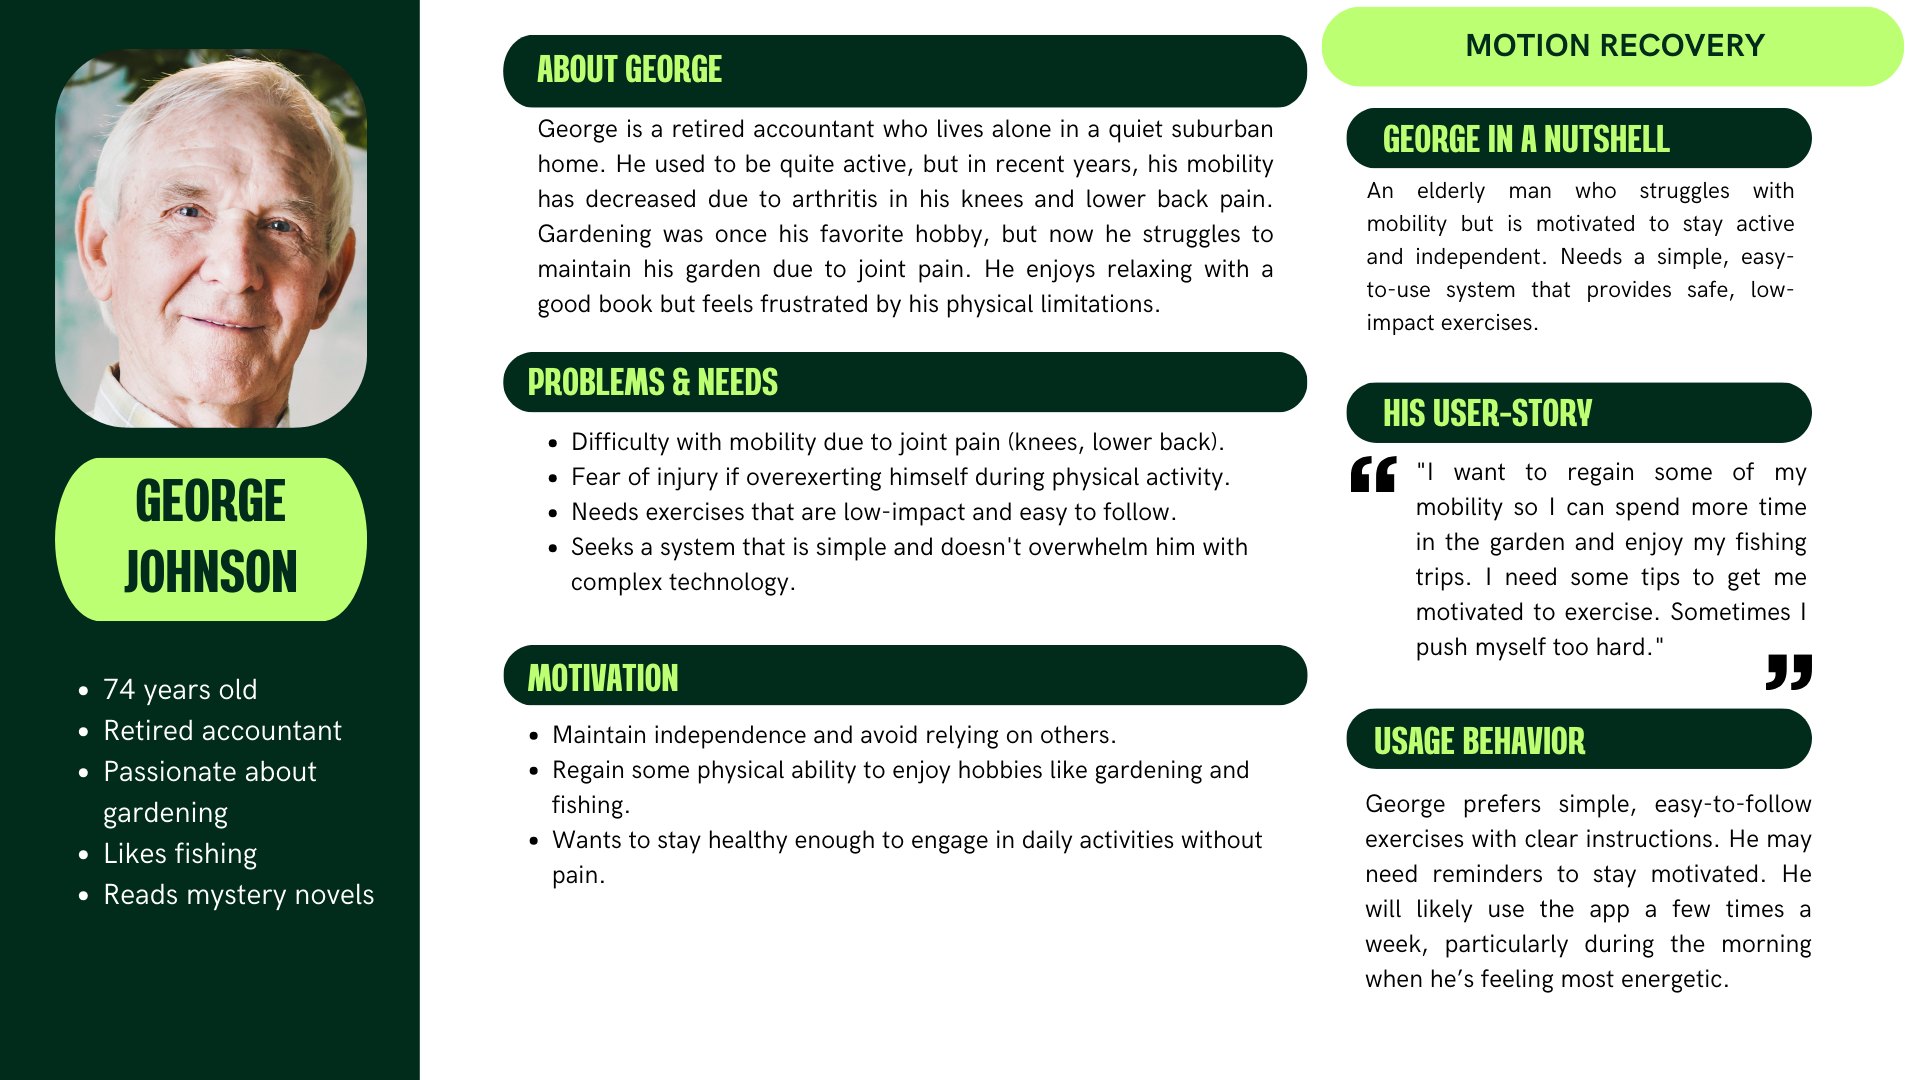
\includegraphics[width=\textwidth]{images/personas/patient_elderly.png}
    \subsubsection{Kids}
    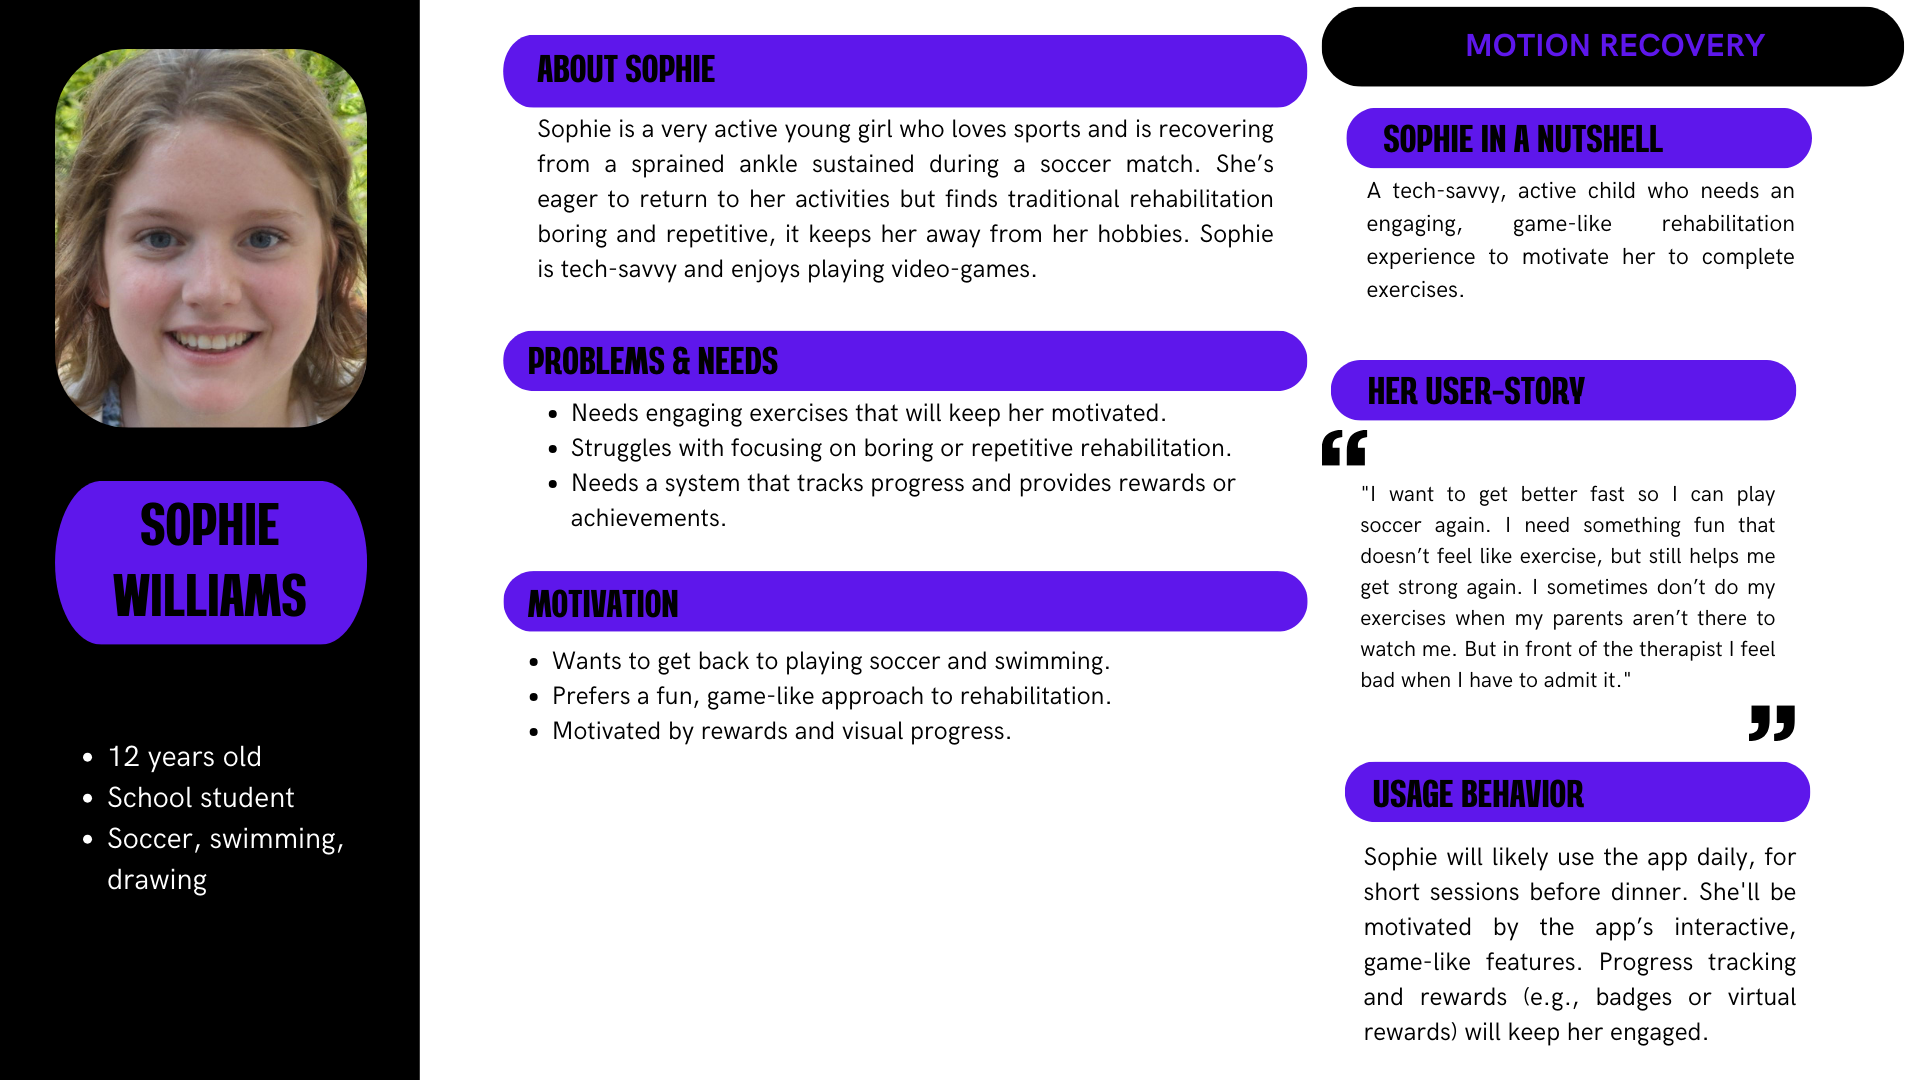
\includegraphics[width=\textwidth]{images/personas/patient_kid.png}
    \subsubsection{Parents of Kids}
    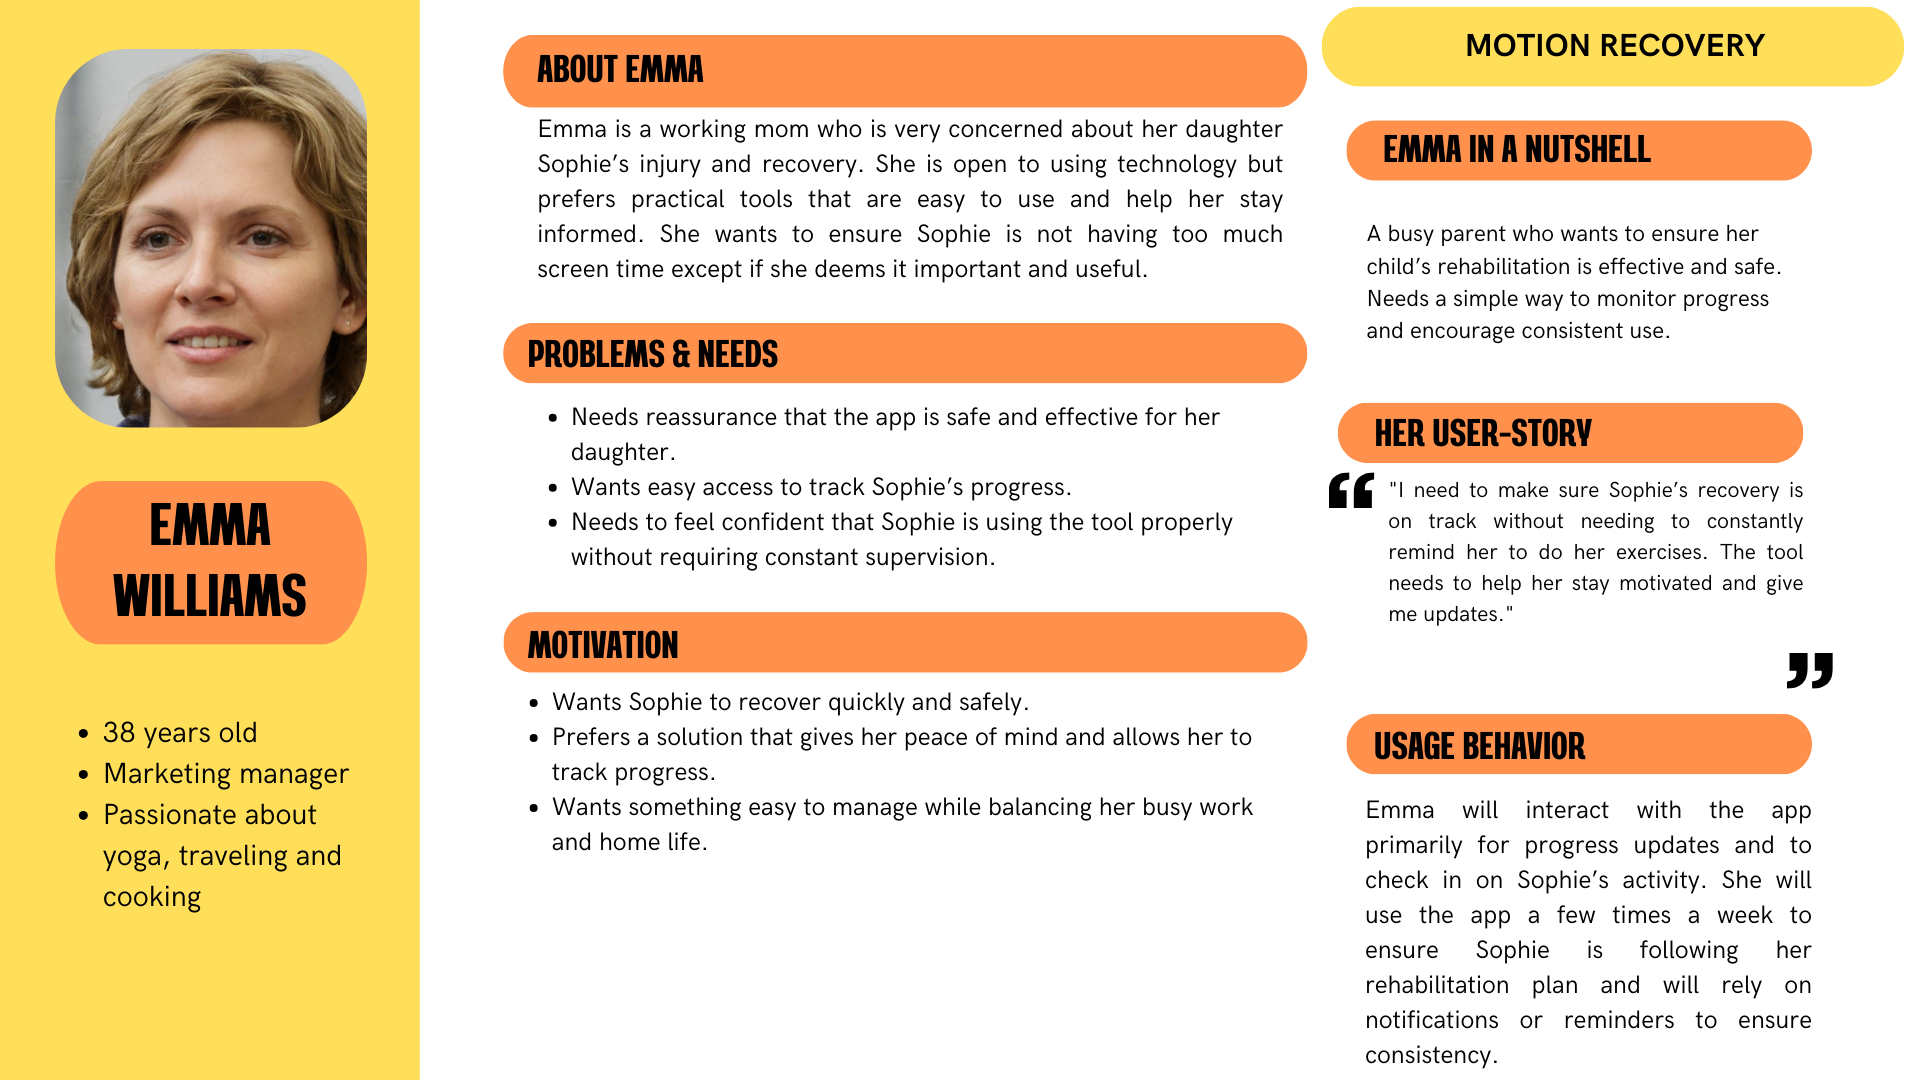
\includegraphics[width=\textwidth]{images/personas/patient_parent.png}
    \subsubsection{Athletes}
    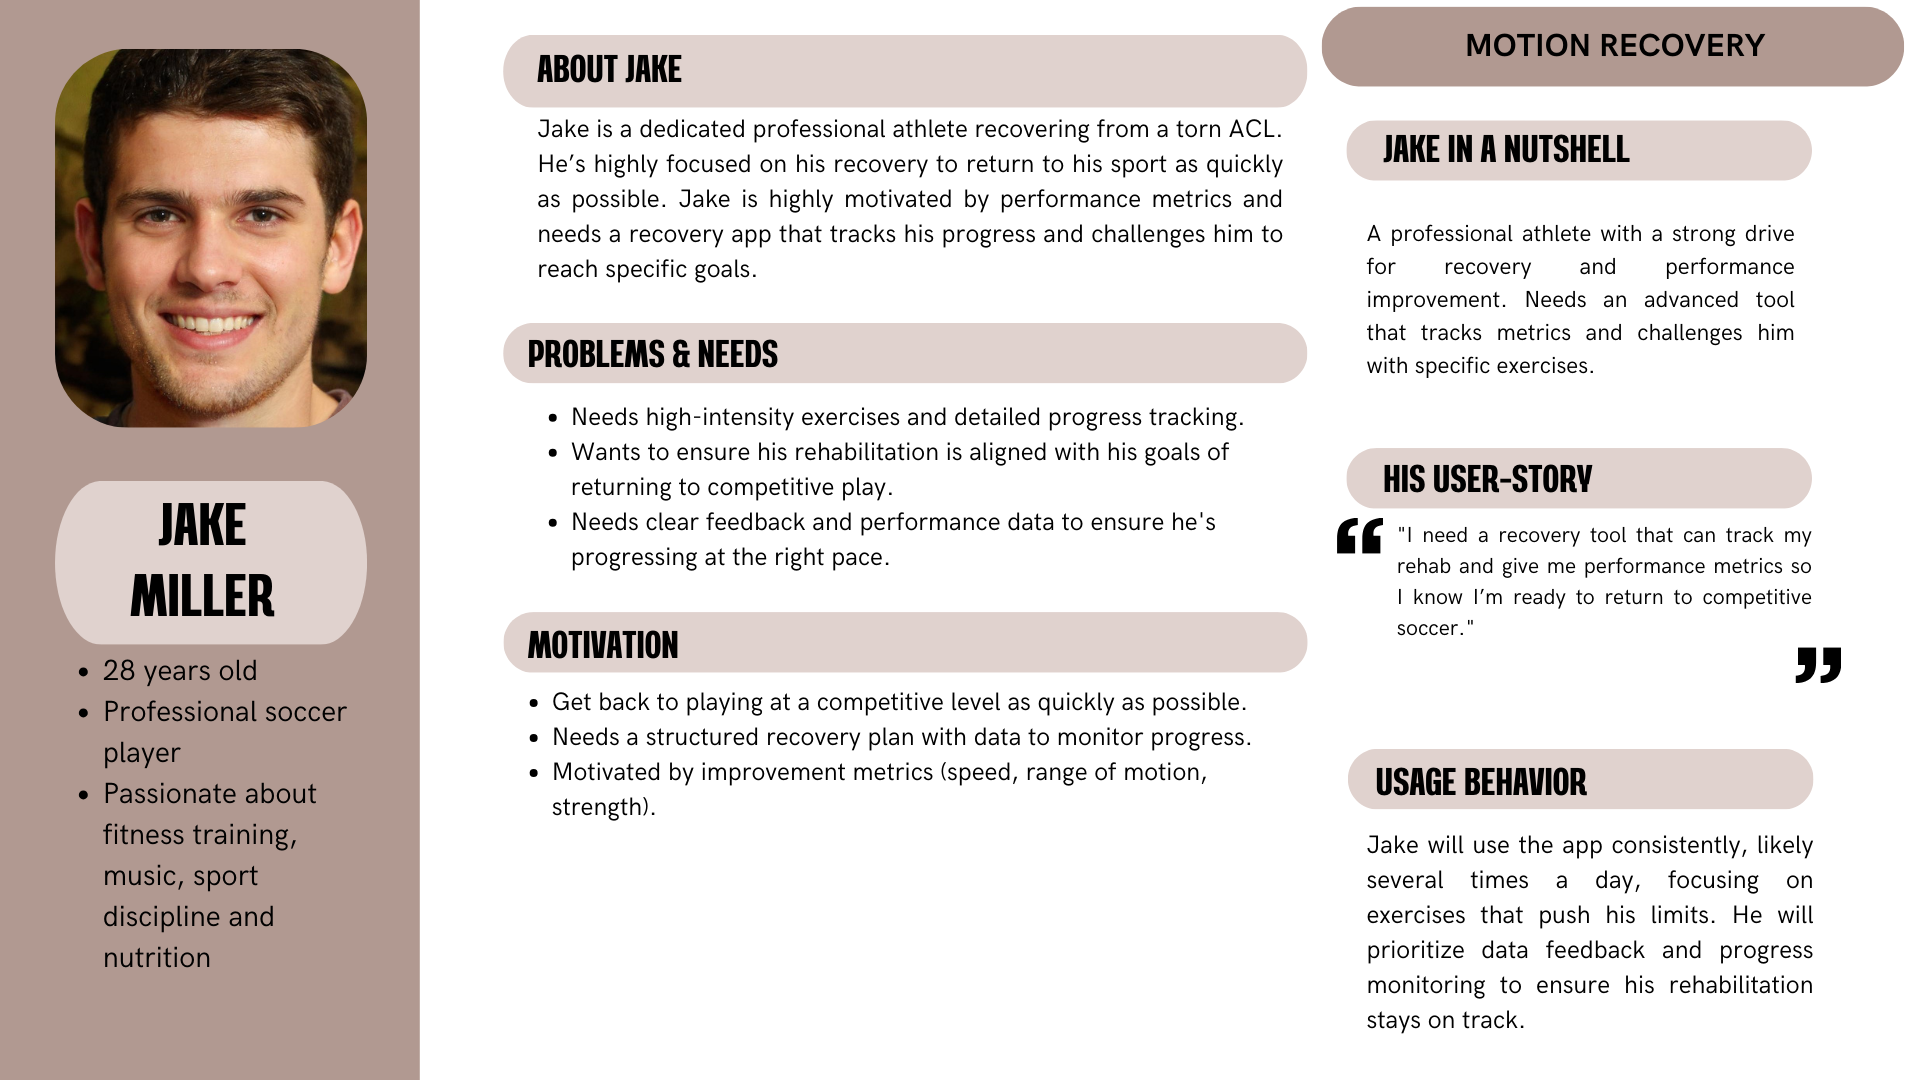
\includegraphics[width=\textwidth]{images/personas/patient_athlete.png}
    \subsubsection{Workers Injured on the Job}
    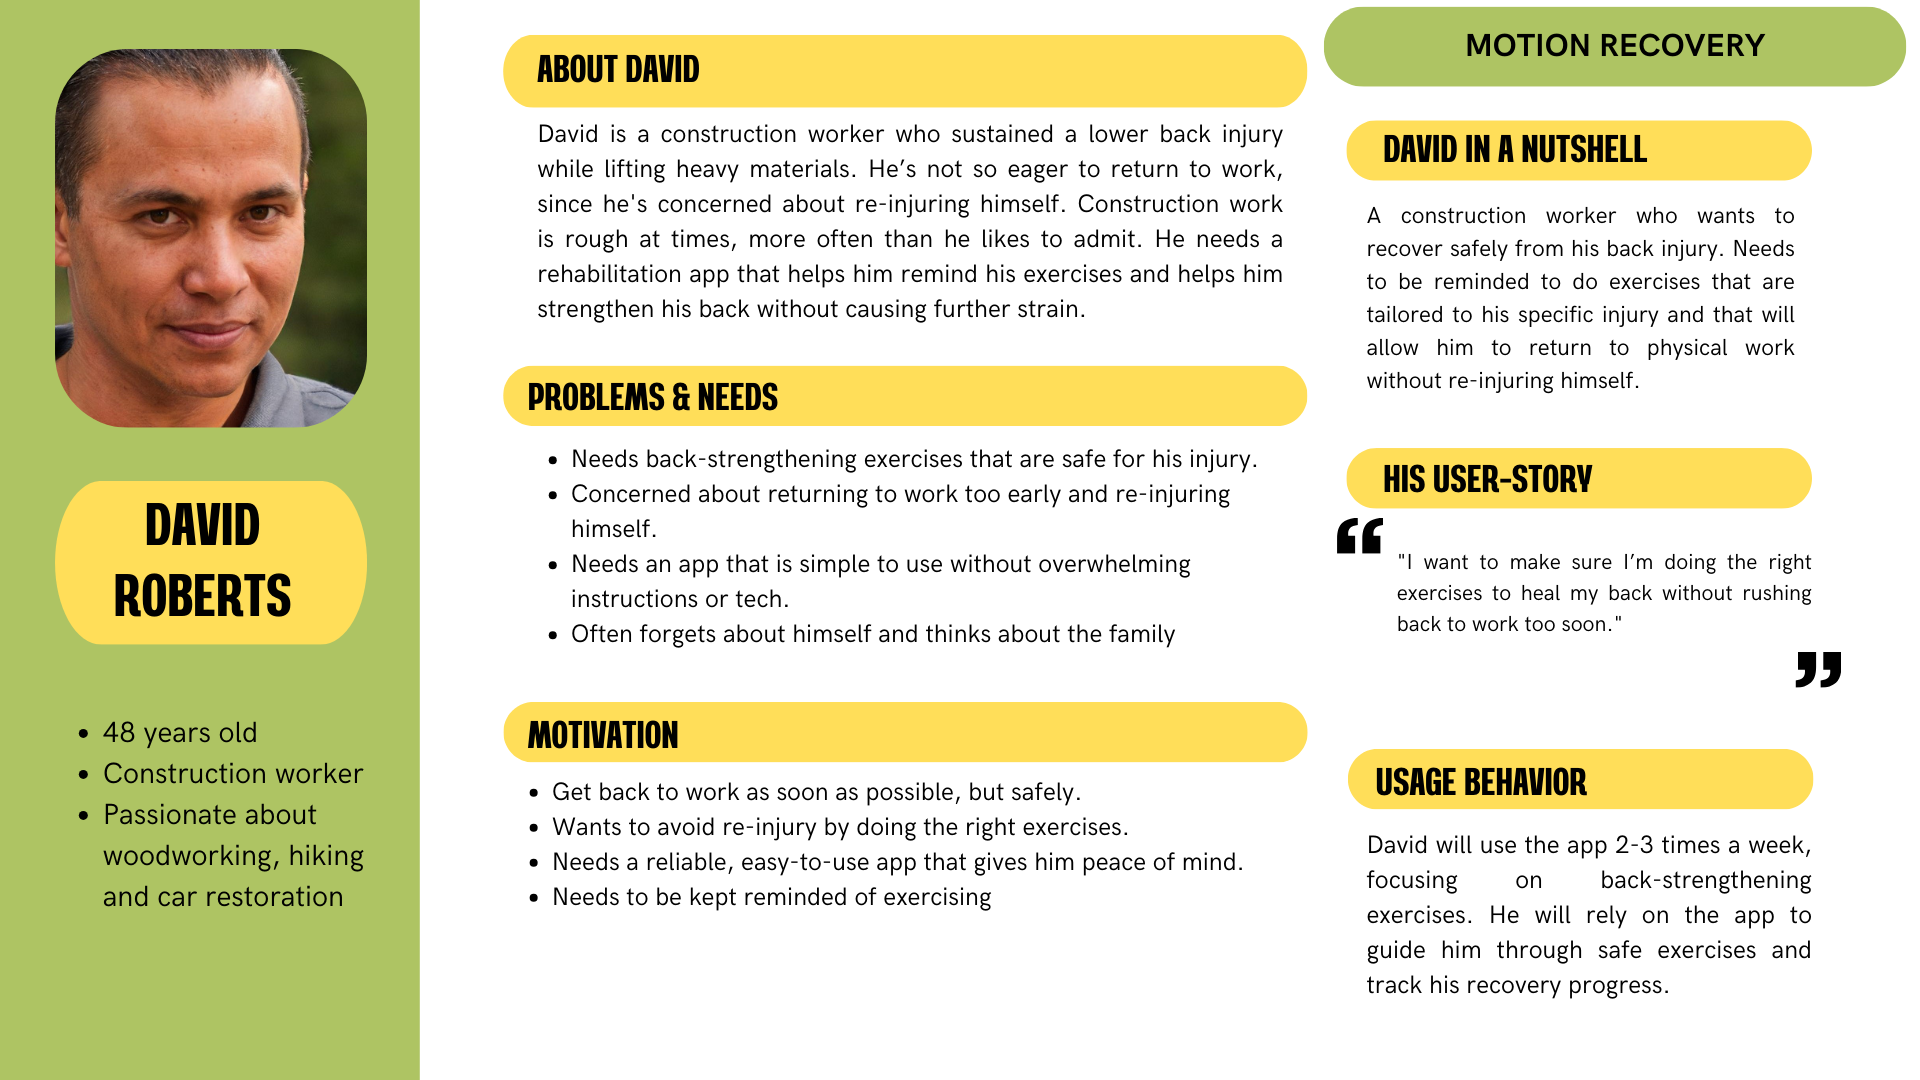
\includegraphics[width=\textwidth]{images/personas/patient_worker_injured.png}
    \subsubsection{Adults with Physical Afflictions}
    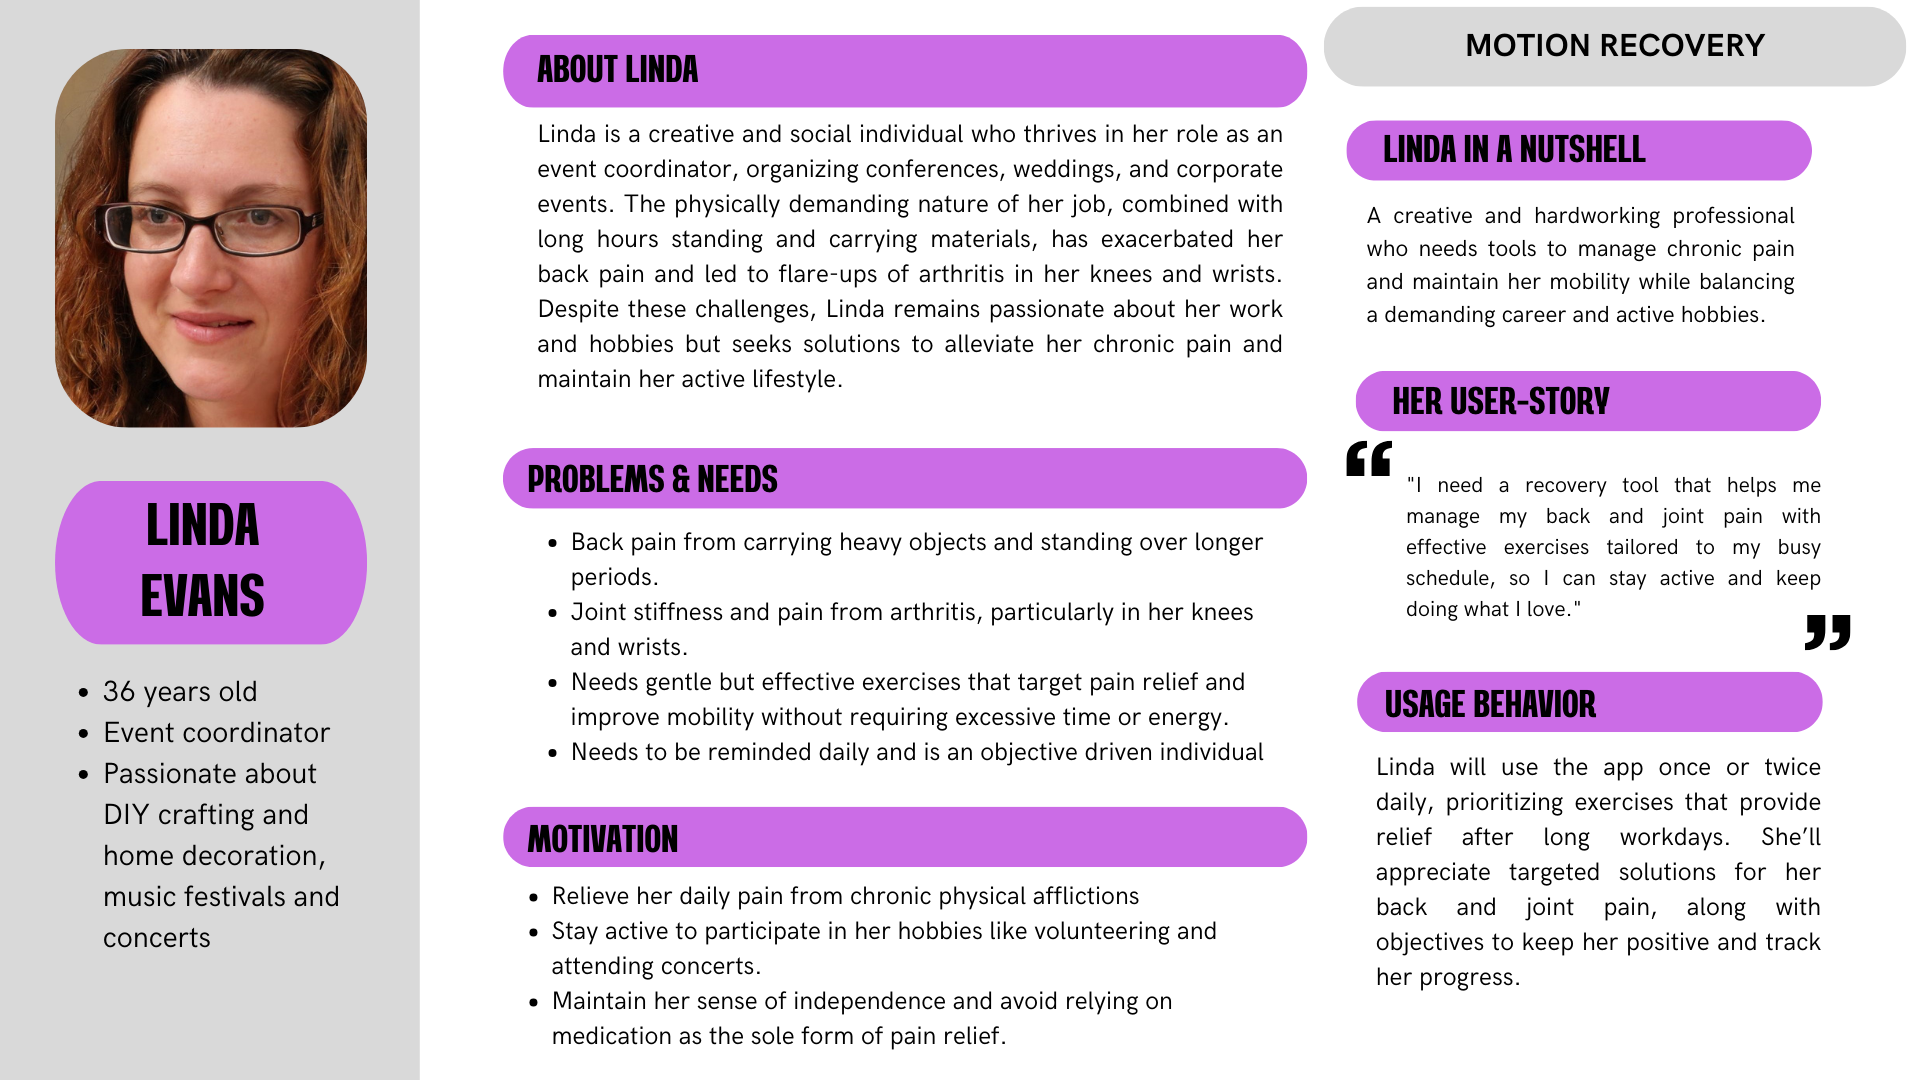
\includegraphics[width=\textwidth]{images/personas/patient_adult_physical_affliction.png}

\subsection{Priorities Assigned to Users}
\subsection{User Participation}
\subsection{Maintenance Users and Service Technicians}
